\chapter{Desenvolvimento}

Para o desenvolvimento do ePuppy foi necessário seguir alguns critérios da Engenharia de Software seguindo alguns pensadores da Área, para facilitar a aplicação e a elaboração de um sistema consistente. Segundo Pessman \cite{Pressman2006}, todo o desenvolvimento de um software é “sistemático, disciplinado e quantificável”, ou seja, precisamos de disciplina, mas também adaptabilidade e agilidade. 
\\
\indent
A princípio, procurou-se reter nas especificidades de uma rede social, aprimorando-se em suas características básicas e em seu comportamento. Após esse momento, foram realizadas pesquisas sobre outros sistemas similares e em quais ambientes o ePuppy poderia se expandir, para não ser apenas uma rede social, um sistema de clínica veterinária ou até mesmo um sistema de segurança para os animais, mas sim, um sistema que englobasse todas essas caraterísticas, tornando-se um projeto mais completo e inovador.
\\
\indent
Após este processo, começou-se uma análise dos requisitos, focada na entrevistas com usuários, workshops e brainstormings de requisitos com donos de clinicas e veterinários, e prototipagens. 
\\
\indent
A medida que foi adquirida uma gama de requisitos, foram realizadas reuniões para definição das ferramentas que seriam utilizadas.
\\
\indent
Em seguida, começou-se a execução da aplicação, elaborando, primeiramente, os usuários que iriam atuar no sistema, a modelagem do banco de dados e criação dos casos de uso. 
\\
\indent
Posteriormente, iniciou-se a implementação, ou seja, toda a etapa de codificação do ePuppy.


\section{Redes Sociais}
A rede mundial, ou {\it Internet} surge em plena guerra fria, com objetivos militares específicos e um importante meio de comunicação acadêmica. Em meados da década de 90 a internet começou a alcançar a população em geral, a com isso surgiu também a utilização de interface gráfica e a criação de sites mais dinâmicos, visualmente mais interessantes.
\\
\indent
A partir dos anos 2000 a conexão entre as pessoas ficou ainda mais fácil e com o aprimoramento desta tecnologia da informação, outro tipo de serviço de comunicação começou a ganhar forças: as {\bf Redes Sociais}. Estrutura social composta por pessoas e organizações, conectadas por vários tipos de relações, que compartilham valores e objetivos comuns, sejam eles, imagens, informações, vídeos e arquivos de áudio.
\\
\indent
Desde 2006, esses serviços viraram “febre” no mundo inteiro chegando a haver uma grande descriminação para aqueles que não usavam.
\\
\indent
Mas como é possível um convívio social à grandes distâncias? Segundo Brown e Barnett, “o agrupamento de indivíduos, de acordo com as posições que resultam dos padrões essenciais de relações de obrigação, constitui a estrutura social de uma sociedade”. Portanto, esses valores unidos aos fatores virtuais, fazem com que haja um estrapolamento das quatro paredes convencionais, tornando assim um convívio social a grandes distâncias.
\\
\indent
Hoje, as principais redes sociais sejam elas profissionais, de relacionamentos, politicas ou comunitárias são: LinkedIn, Myspace, Facebook, Twitter, entre outros.

\section{ePuppy}
O ePuppy surge como um projeto designado para quem procura mais praticidade em questão de segurança, informação e interação. Para que isso fosse precisamente implementado no sistema subdividiu-se os três quesitos em vários casos de uso.
\\
\indent
O sistema funcionará com basicamente três tipos de usuários (Proprietários, clínicas e veterinários). E disponibilizando as mais variadas tarefas para esses usuários, passando de controle e segurança de animais dos proprietários, até ao controle de proprietários e veterinários em clínicas veterinárias.
\\
\indent
Os proprietários do sistema poderão cadastrar seus animais, adicionando nomes, espécie, raça dentre outros dados. Cada animal será identificado por um {\it QR Code} diferenciado, na qual, a priori, serão adicionadas em coleiras, dependendo do animal. O {\it QR Code} terá dados acerca do dono e do pet, garantindo assim, que o proprietário seja facilmente notificado, por quem achar o animal (caso este esteja perdido). Os {\it pets} ainda terão um histórico hospitalar, para que os veterinários permitidos pelo dono, tenham todo um apanhado detalhado de suas consultas passadas, obtendo assim: Remédios, consultas, cirurgias e doenças acerca do animal.
\\
\indent
Por o ePuppy ser um sistema de segurança e também, uma rede social, os usuários em geral poderão compartilhar publicações como: informações e arquivos em geral, comentar publicações, ter amigos, grupos, ver perfis de outros usuários e seus animais. Além de todos esses atributos, o sistema ainda disponibilizará aos usuários, {\it login} por redes sociais, fazendo com que publicações e ações em relação aos seus animais, clínicas e veterinários, sejam publicadas também nessas outras redes, caso o usuário atribua permissão para tal procedimento.
\\
\indent
Já do lado das clínicas veterinárias, o ePuppy procura proporcionar meios para que essas divulguem os seus serviços, na própria rede social e em outras, além de possibilitar um maior controle de seus pacientes e veterinários, outrossim, uma maior facilidade de acesso dos usuários.
\\
\indent
A rede social ainda possibilita um auxílio ao trabalho dos veterinários, principalmente porque esses terão um maior acesso às antigas consultas de seus pacientes (animais), podendo ser mais eficientes durante o receitamento de determinado remédio, consulta, cirurgia, além de um maior monitoramento desses.

\section{Trabalhos Relacionados}
Para o desenvolvimento do ePuppy, tomou-se como base um sistema que já está em funcionamento, chamado Meu Peludo, disponível no site (http://www.meupeludo.com.br/). Nele, o proprietário compra a coleira do sistema, que contém um {\it QR Code} agregada a um {\it link} da {\it internet}, que contém os dados do animal, do dono e um formulário, para o preenchimento da pessoa que encontrar o animal (caso este esteja perdido), fazendo com que este consiga entrar em contato com o dono. %Nos apoiamos nessa funcionalidade em especial, e fomos aderindo novas, buscando deixar o ePuppy mais completo e mais amplo.
\\
\indent
Durante o desenvolvimento da mais nova rede social, conheceu-se um sistema chamado TagPet, disponível em (https://www.tagpet.com.br/), que tem muitas das funcionalidades que o ePuppy conteria, principalmente, o histórico hospitalar e os dados do animal a partir do Qr Code. Porém, a ideia do projeto é ser uma rede social para proprietários de animais domésticos, disparando suas publicaçõs nas demais redes sociais do usuário, caso ele tenha se cadastrado utilizando os dados destas. Além disso, as pessoas poderão compartilhar em quais clínicas ou {\it pet shops} favoritos estão, funcionando como uma publicidade para esses lugares.


\section{Análise dos Requisitos}
O levantamento de requisitos para a construção do ePuppy foi de extrema importância, pois compreender de maneira correta e eficaz as necessidades dos usuários, é o alicerce para um sistema consistente. 
\\
\indent
Mesmo conhecendo a variedade de redes sociais disponíveis, não era o suficiente para a elaboração do projeto, por ele não se limitar apenas a uma rede social comum, mas englobar donos de animais de estimação, clínicas veterinárias, veterinários e empresas de produtos e serviços.
\\
\indent
Portanto, devido a falta de conhecimento necessário da área a ser desenvolvido o projeto, foi fundamental obter o máximo de requisitos possíveis. Os requisitos de um sistema são descrições dos serviços fornecidos pelo sistema e as suas restrições operacionais, ou seja, refletem a necessidade do cliente \cite{Sommerville2011}.


\subsection{Elicitação de Requisitos}
Para Pressman \cite{Pressman2006}, entender os requisitos de um problema está entre as tarefas mais difíceis enfrentadas por um engenheiro de software, porque surpreendentemente, na maioria dos casos, o cliente não sabe o que é necessário, e não tem um bom entendimento das características e funções que vão oferecer benefícios.
\\
\indent
Por conhecer bem que o levantamento de requisitos não é uma tarefa fácil, devido a dificuldades que os usuários tem de descrever o problema ou até mesmo, pela possibilidade de haver contradições de ideias entre usuários e analistas, utilizou-se técnicas padrões usadas na Engenharia de Software. Abaixo, seguem algumas das técnicas utilizadas na elicitação dos requisitos:
\begin{itemize}
   \item Entrevistas com usuários:
   \\
   \indent
   Por ser um método tradicional e que geralmente constrói bons resultados, os mais variados tipos de usuários foram entrevistados, principalmente, veterinários e donos de animais. 
   \item {\it Brainstorming}:
    \\
   \indent
   O {\it Brainstorming} foi outro método utilizado e que também rendeu bons resultados. Foi realizada principalmente entre veterinários, pois poderiam contribuir da melhor forma possível, por viver no ambiente cotidianamente. 
   \item Estudo Etnográfico:
   \\
   \indent
   Em conjunto com os {\it Brainstormings} e entrevistas com usuários, realizou-se o estudo baseado na observação, para compreender o ambiente e o contexto onde o sistema será inserido.
   \item Prototipagem: 
   \\
   \indent
   Para a demonstração do andamento do projeto, apresentou-se protótipos com algumas funcionalidades, principalmente para as clinicas e veterinários, para que essas começassem a se familiarizar com o sistema e divulgá-lo aos seus clientes.
   \item Workshops de requisitos:
   \\
   \indent
   Além de todos os métodos utilizados anteriormente, também efetuou-se várias reuniões estruturadas com veterinários, clinicas e investidores, a fim de modificar, adicionar ou esclarecer os requisitos.
 \end{itemize}
 
\subsection{Diagrama de Casos de Uso}
Os casos de uso descrevem as principais funcionalidades do sistema e a interação dessas com os demais usuários, não aprofundando em detalhes técnicos, ou seja, não descreve como o sistema realiza tais funções.
\\
\indent
A partir dos casos de uso, podemos identificar uma sequência de eventos que acontece quando um usuário interage com o sistema (Cenário), usuários do sistema (Atores), funcionalidades realizadas pelos atores ({\it Use Case}) e a comunicação, que será basicamente o que liga um ator a um caso de uso. Abaixo, estão demonstrados os casos de uso, subdivididos em módulos:


\begin{figure}[h!]
	\centering	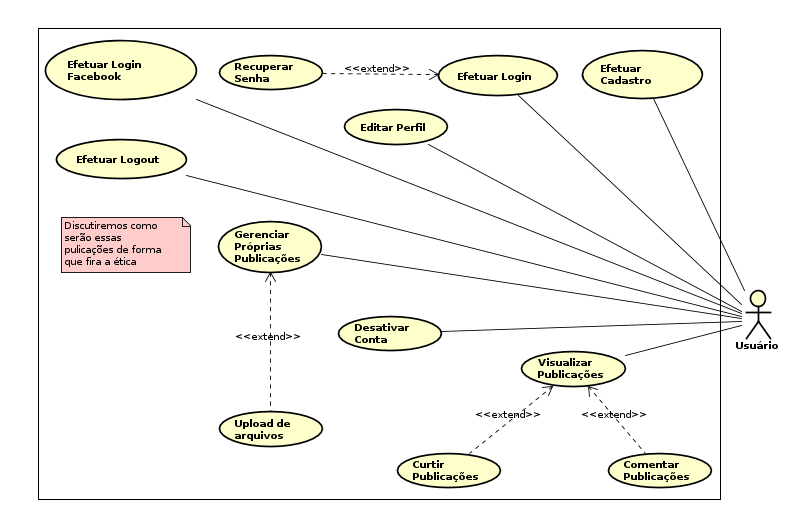
\includegraphics[scale=0.50
	]{imagens/usercasodeuso}
	\caption{Módulo usuário}
	Fonte: Autoria Própria.
	\label{Rotulo}
\end{figure}

\newpage
A Figura 2, ilustra as ações que poderão ser realizadas por todos os usuários (proprietários, veterinários e clinicas), expondo ,principalmente, a efetuação de cadastro, {\it login} e {\it logout}, edição de perfil e o gerenciamento (adição, edição e exclusão) de publicações.


\begin{figure}[h!]
	\centering	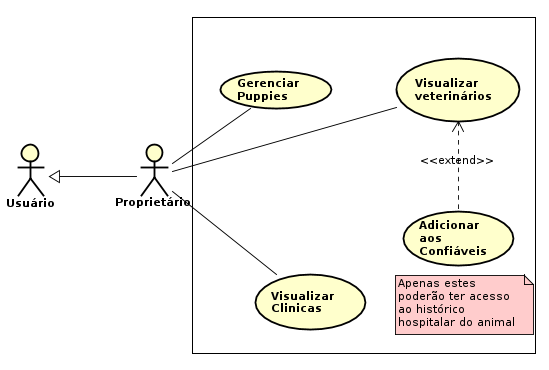
\includegraphics[scale=0.50
	]{imagens/ownerscasosdeuso}
	\caption{Módulo Proprietário}
	Fonte: Autoria Própria.
	\label{Rotulo}
\end{figure}
\newpage
Na Figura 3, são apresentadas as ações restritas aos donos dos animais, especialmente, o gerenciamento dos puppies (animais) e a adição dos veterinários aos seus confiáveis. Além disso, também é evidenciado a herança entre proprietário e usuário, na qual, o primeiro poderá realizar todas as operações do segundo.


\begin{figure}[h!]
	\centering	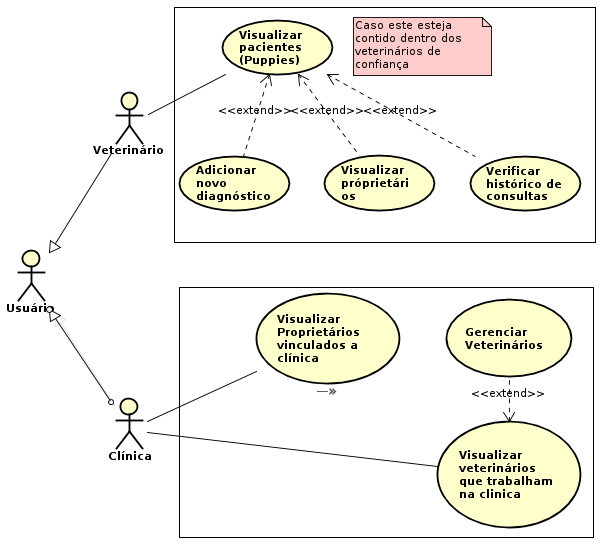
\includegraphics[scale=0.50
	]{imagens/HeVcasosdeuso}
	\caption{Módulos Veterinário e Clínica}
	Fonte: Autoria Própria.
	\label{Rotulo}
\end{figure}


São ilustrados na figura 4 todas as operações que poderão ser realizadas pelos veterinários e clínicas. Os veterinários poderão adicionar novos diagnósticos e a verificar o histórico hospitalar dos animais em que estes são vinculados. Já as clínicas poderão visualizar seus pacientes (animais) e seus donos, além de gerenciar os veterinários. Assim como os proprietários, ambos herdam as ações do usuário.

\subsection{Diagrama Entidade-Relacionamento}
O Diagrama de Entidade e Relacionamento descreve toda estrutura lógica do banco de dados,  ou seja, representa de forma abstrata a estrutura que possuirá o banco da aplicação.
\\
\indent
A partir de modelo pode-se descrever os objetos (Entidades) envolvidos em um domínio de negócio, suas caraterísticas (atributos) e seus relacionamentos.

\begin{figure}[h!]
	\centering	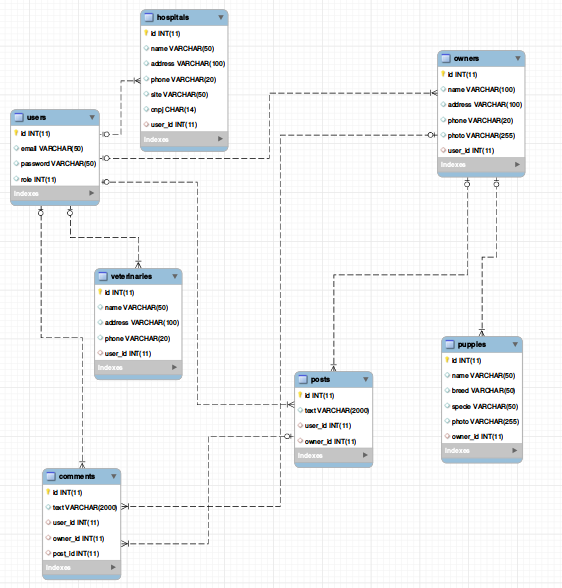
\includegraphics[scale=0.80
	]{imagens/entidaderelacionamento}
	\caption{Diagrama Entidade-Relacionamento}
	Fonte: Autoria Própria.
	\label{Rotulo}
\end{figure}

A figura acima (Figura 5), representa o diagrama de Entidade-Relacionamento que possui ao todo 7 tabelas: hospital (clinicas), users (usuários), owners (proprietários), puppies (animais), veterinaries (veterinários), posts (publicações) e comments (comentários). 
\\
\indent
A tabela users está diretamente relacionada com os trés tipos de usuários do sistema: owners, hospitals e veterinaries, na qual, a ligação entre eles é de 1 para 1, ou seja, um user poderá identificar apenas um owner e assim por diante. 
\\
\indent
A tabela owner está relacionada com puppies, posts e comments. Todas são interligadas com ligação de 1 para N, na qual, um proprietário poderá cadastrar quantos animais desejar, criar várias publicações e comentá-las,  a medida que pretender e necessitar.
\\
\indent
Algumas tabelas ainda não foram adicionadas devido a alguns problemas com alguns requisitos que foram modificados recentemente.

\section{Metodologia}
Para a produção de um software de alta qualidade, engenheiros de software procuram a maneira mais eficaz, adotando uma abordagem sistemática e organizada em seu trabalho. \cite{Sommerville2011}.
\\
\indent
No entanto, a engenharia de software seleciona métodos mais apropriados para um conjunto de circunstâncias e uma abordagem mais criativa e menos formal, sendo fortemente eficaz. \cite{Sommerville2011}.
\\
\indent
Dessa forma, a engenharia de software utiliza uma tecnologia de camadas, apoiando-se num compromisso organizacional com a qualidade. A partir disso, tem-se o alicerce dessa camada, denominada camada de processo que define a metodologia que devem ser estabelecidos para a efetiva utilização da tecnologia da engenharia de software. Após o processo, tem-se os métodos que fornecem a técnica de “como fazer” para a construção de softwares e por fim, a ferramentas que fornecem apoio automatizado ou semi-automatizado para o processo e para os métodos. \cite{Pressman2006}.
\\
\indent
O ePuppy foi desenvolvido na linguagem de programação PHP (um acrônimo recursivo para {\it PHP: Hypertext Preprocessor}, originalmente Personal Home Page), disponível no site (www.php.net), na versão 5.5.9.
\\
\indent
Criada em 1995 por Rasmus Lerdorf, é uma linguagem interpretada usada para criação de aplicações que executam no lado do servidor, capazes de gerar conteúdo dinâmico em páginas que utilizam linguagem de marcação HTML (em acrônimo para {\it HyperText Markup Language}). A vantagem é que páginas HTML \cite{Freeman2006} podem ser interpretadas por navegadores {\it web} tradicionais, como por exemplo: Firefox, Chrome, Internet Explorer, Safari ou Opera.
\\
\indent
O esforço de desenvolvimento do projeto foi minimizado com a utilização do {\it framework} CakePHP, disponível no site (www.cakephp.org), na versão 2.5.5. 
\\
\indent
Um {\it framework}, em linhas gerais, é uma abstração que une códigos comuns entre vários projetos de software provendo uma funcionalidade genérica, que pode atingir uma funcionalidade mais específica, por configuração, durante a programação de uma aplicação. O CakePHP foi desenvolvido em 2009 por Garrett Woodworth. É escrito na linguagem de programação PHP e tem como principais objetivos oferecer uma estrutura que possibilite aos programadores de todos os níveis, contemplando os alunos iniciantes do instituto federal, desenvolverem aplicações robustas rapidamente, mas sem perder flexibilidade.
\\
\indent
A escolha foi motivada pelo fato do CakePHP utilizar conceitos de Engenharia de Software e Padrões de Projetos bem-conhecidos
\cite{Gamma1994} e
\cite{Fowler2003}, tais como: {\it Active Record, Association Table Mapping, Front Controller e Model-View-Controller (MVC)}.
\\
\indent
Os dados dos usuários (Proprietários, clinicas e veterinários), animais, plublicações, históricos de consultas, e-mails entre outras, funcionam on-line e os esses são guardados de forma segura no banco de dados MySQL, disponível no site (www.mysql.com), na versão 5.5.43. 
\\
\indent
O MySQL foi desenvolvido em 1995 por David Axmark, Allan Larsson e Michael Monty, e utiliza a linguagem de consulta SQL (um acrônimo para {\it Structured Query Language}) como interface. Vários motivos nos levaram a escolha desse banco de dados, dentre eles: integração nativa com a linguagem PHP, excelente desempenho, estabilidade e suporte para qualquer plataforma atual \cite{Suehring2002}.
\\
\indent
Para o controle de versionamento do sistema, utilizamos o Git, disponível no site (www.git-scm.com), na versão 2.6.2. 
\\
\indent
Um sistema de controle de versão com a possibilidade de gravar documentações e comentários. O Git foi desenvolvido inicialmente por Linus Torvalds em 2005 com a finalidade de versionalizar projetos visando uma maior, velocidade, {\it design} simples, com Suporte robusto a desenvolvimento não linear (milhares de {\it branches} paralelos), distribuído e capaz de lidar eficientemente com grandes projetos como o {\it kernel} do Linux (velocidade e volume de dados).
\\
\indent 
Em conjunto com o Git, utilizamos o BitBucket em sua versão gratuita, encontrado no {\it link} (www.bitbucket.org).
\\
\indent
 É um site que visa hospedar projetos, utilizando o Git como o controlador de versão. O BitBucket foi desenvolvido em 2008 com Python. A escolha foi motivada pelo fato do BitBucket disponibilizar uma versão gratuita com espaço ilimitado e com capacidade para 5 programadores, caso o projeto seja privado, se não, o bitbucket também disponibiliza quantidade ilimitada de programadores.
\\
\indent
	Toda a codificação do projeto foi desenvolvida com a utilização dos editores, Atom (versão 1.0) e Brackets (1.0).
\\
\indent
O Atom é um editor de código fonte livre e de código aberto para OS X, Linux e Windows e foi desenvolvido em 2014 pela GitHub. A escolha pelo editor foi incentivada pelo fato de suporte para plugins escritos em Node.js e principalmente pela incorporação de controle Git, mostrando os arquivos modificados de acordo com o Git.
\\
\indent
O Brackets é um editor de texto open source e moderno, para criação e edição de arquivos (IDE) HTML, CSS, JS e PHP. Foi desenvolvido pela Adobe e tem como principais atributos, atualizações em tempo real (quando em conjunto com o Chrome), instalador de extensão e possibilidade de personalização de recursos.
\\
\indent
Uma vez escolhidas as tecnologias a serem utilizadas, foi então organizado o ambiente de desenvolvimento. O projeto foi desenvolvido em 3 computadores pessoais ({\it notebook}) e 3 computadores de mesa ({\it desktop}), no laboratório de pesquisa de informática do campus Natal – Zona Norte. Os {\it notebooks} tinham processadores Intel Core i5, 4 GB de memória RAM, executando o sistema operacional Linux, distribuição Ubuntu, Voyager ou Arch Linux. Os computadores pessoais tinham processadores AMD Athlon, 4 GB de memória RAM, executando o sistema operacional Windows 7.	
\\
\indent
O processo de construção do sistema ePuppy foi realizado sempre com a divisão de grupos, denominados {\it Back-End} (responsáveis pela codificação e interligação dos códigos com a interface) e {\it Front-End} (Responsáveis pela criação da interface). A codificação do sistema foi totalmente distribuída em pares, na qual, duas pessoas codificam as mesmas coisas, amenizando os erros que podem ocorrer durante o processo devido a permanente inspeção de código que ocorre durante seu uso.
\\
\indent
Além dessa divisão, segmentou-se a construção do ePuppy em cinco etapas (Sommerville, 2011): (I) levantamento de requisitos, (II) modelagem, (III) codificação, (IV) teste e (V) implantação. Porém, o andamento do projeto está entre as etapas (III) e (IV), ou seja, as etapas de codificação e testes dos códigos que estão sendo projetados.
\\
\indent
	A etapa (I), foi dedicada ao entendimento das necessidades de um cliente em potencial, bem como, foi estudada a viabilidade de desenvolvimento do projeto. Foram realizados entrevistas e a formulação de questionários com dois profissionais da área e com proprietários de animais, para que pudéssemos realizar o levantamento dos requisitos necessários para a formação da ideia. Uma vez alcançado um entendimento geral do projeto, foram conduzidas reuniões com os mesmos profissionais para validar as especificações levantadas, e então definir uma especificação final isenta de ambiguidades, para a produção do relatório final da etapa (Documento de Requisitos). Os questionários e documento final foram elaborados utilizando apenas o editor de texto LibreOffice Writer, disponível no site (www.libreoffice.org), na versão 4.2.8.2.
\\
\indent
Já na etapa (II), uma vez que foram definidos os requisitos funcionais e não-funcionais do sistema, foi dado início à modelagem. Em outras palavras, foram produzidos os diagramas de caso de uso e de classe \cite{Fowler2005} e \cite{Bezerra2002}. O primeiro diagrama permite literalmente, desenhar o processo de execução do negócio e visualizar a responsabilidade de cada participante (atores), quando ele entrará em cena, qual a sua interação, a amplitude e a sequência em que seu trabalho precisa ser realizado em relação às responsabilidades e tarefas dos demais integrantes do processo. O segundo diagrama faz uma representação da estrutura e relações das classes que servem de modelos para os objetos. Para a construção dos diagramas, foi utilizado o editor Astah, disponível no site (www.astah.net), na versão 7.0.0.
\\
\indent
Na etapa (III), foi realizada a escrita efetiva do programa. Foi utilizado os editores de textos Atom e Brackets para codificação, disponíveis nos sites (www.atom.io) e (www.brackets.io), nas versões 1.0. Cada versão do programa foi controlada e gerenciada com o uso do programa Git, disponível no site (www.git-scm.com), na versão 2.6.2. Para permitir o desenvolvimento colaborativo entre os programadores, o projeto utilizou o serviço de {\it web hosting} do Bitbucket (https://usuário@bitbucket.org/epuppyteam/epuppy.git).
\\
\indent
A etapa (IV) foi dedicada a analisar todo o projeto na tentativa de encontrar possíveis falhas de codificação, a fim de fornecer informações sobre a qualidade do produto em relação ao contexto em que ele deve operar. Os aspectos de qualidade inicialmente investigados foram: funcionalidade e usabilidade. Nos testes de funcionalidade, são criados testes automáticos de unidade com PHPUnit, disponível no site (www.phpunit.de), na versão 4.7, na tentativa de se verificar as menores unidades de software (sub-rotinas, métodos, classes ou pequenos trechos de código). O objetivo do teste é encontrar falhas de funcionamento dentro de uma pequena parte do sistema funcionando independente do todo. Já em relação à usabilidade, analisamos a capacidade do produto ser facilmente compreendido, seu funcionamento aprendido, ser operado e atraente ao usuário. Os testes de usabilidade são realizados com usuários em potencial do sistema, a partir de protótipos ou na própria aplicação sendo executada no ambiente de desenvolvimento.
\\
\indent
Por fim, a etapa (V) disponibilizará o sistema ePuppy em produção para ser utilizado efetivamente. Para essa etapa, será primeiramente realizado o registro do domínio. Em seguida, o sistema será hospedado, num serviço que suporte as tecnologias PHP e MySQL, facilitando o gerenciamento do sistema de forma {\it on-line}. Assim o ePuppy estará pronto para ser acessado pelos demais usuários.

\section{Análise dos Resultados}

O ePuppy conta com segurança de permissão, que garante que os usuários só naveguem no sistema através da interface gráfica, impedindo alguma falha de segurança da informação, caso os mesmos tentem navegar pela url impedindo a entrada caso não encontrem-se logados, por exemplo, a medida que um usuário tentar burlar o sistema adicionando seu numero de identificação (id) na barra de busca, tentando assim, ter acesso aos seus dados, este é imediatamente redirecionado para a tela de login, como ilustrado na Figura 6.

\begin{figure}[h!]
	\center	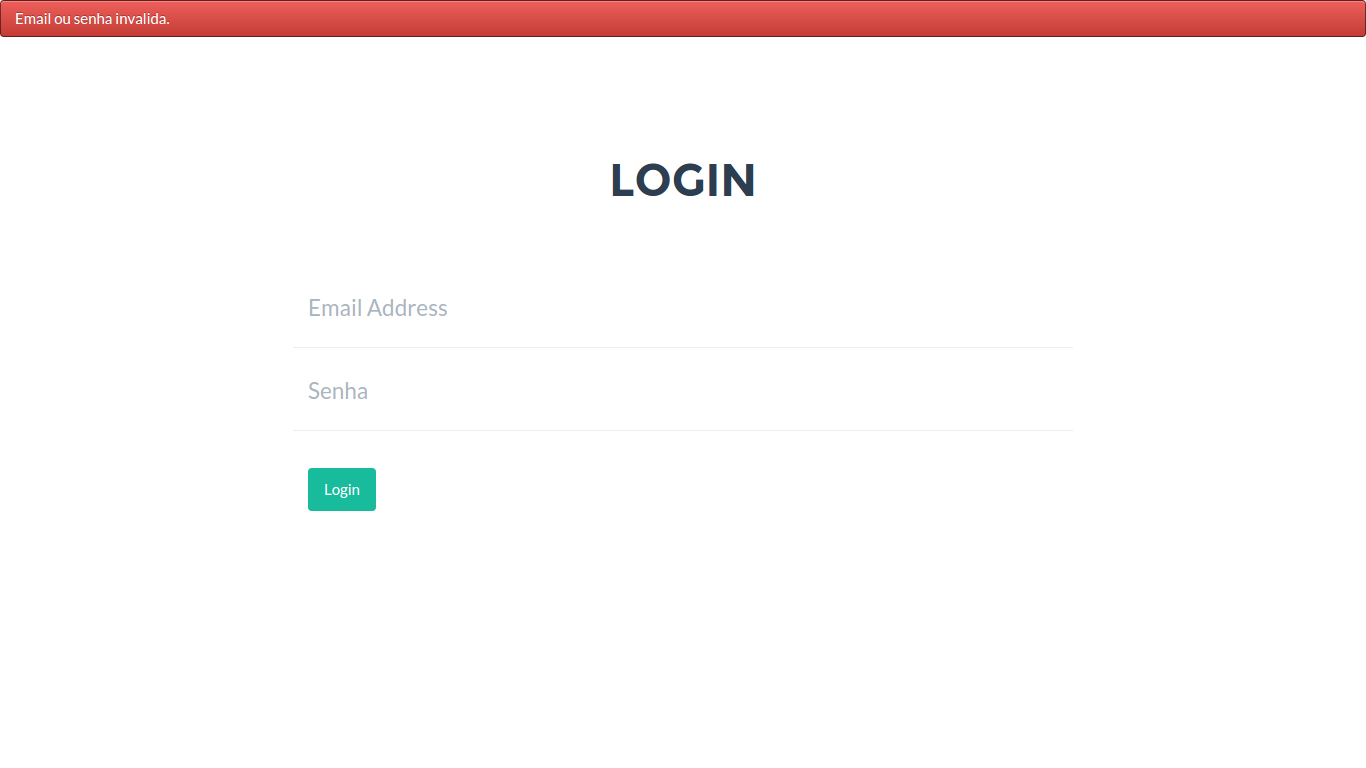
\includegraphics[scale=0.30
	]{imagens/errologin}
	\caption{Página de Login com falha na autenticação}
	Fonte: Autoria Própria.
	\label{Rotulo}
\end{figure}


A página inicial do projeto (Figura 7) conta com uma fácil navegação e simplicidade, assim otimizando o tempo do usuário durante o {\it login}. Dentro desta página há recursos como cadastrar, desenvolvedores e as funcionalidades que poderão ser encontradas através da rolagem da página ou escolhidos no menu superior, fazendo com que o site inicial seja completamente integrado e interativo, como mostrado nas Figuras 7 e 8.
\begin{figure}[h!]
	\center	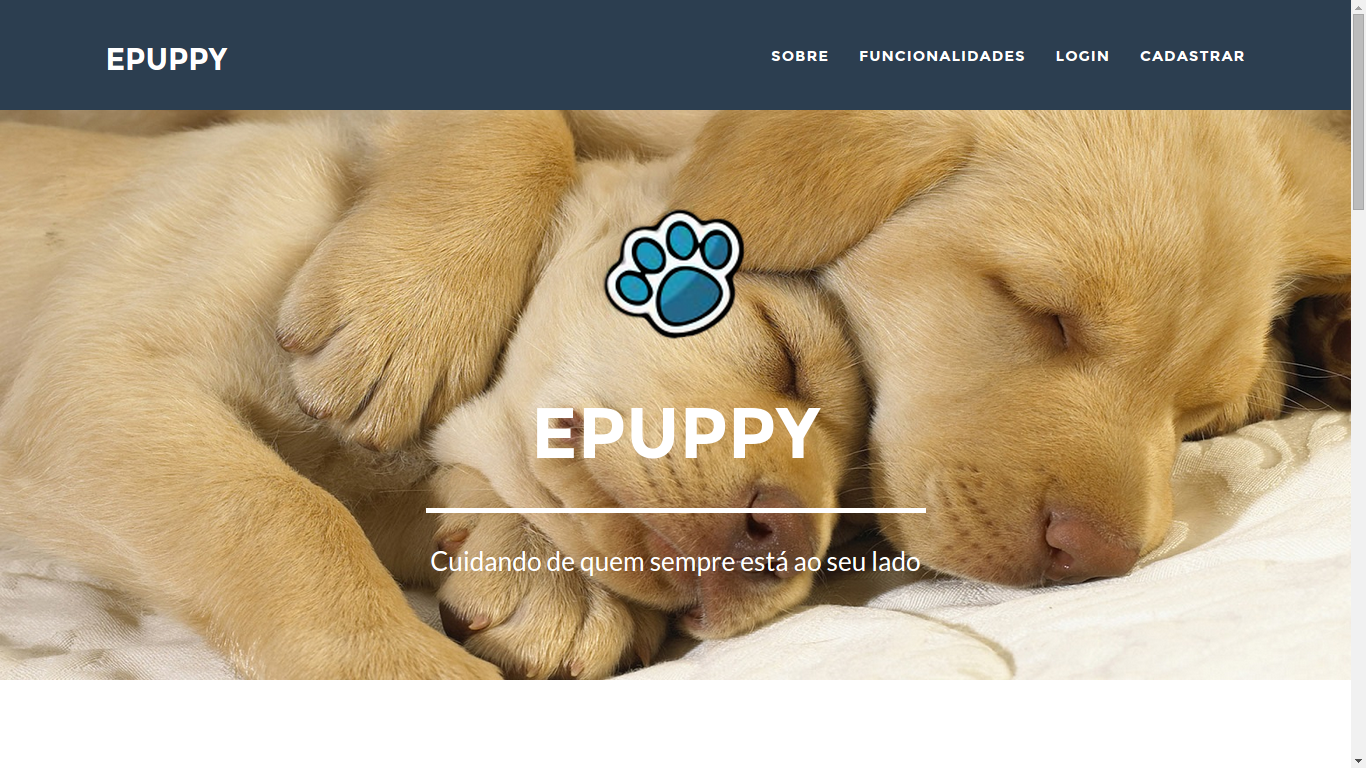
\includegraphics[scale=0.25
	]{imagens/principal}
	\caption{Página home do ePuppy}
	Fonte: Autoria Própria.
	\label{Rotulo}
\end{figure}
\begin{figure}[h!]
	\center	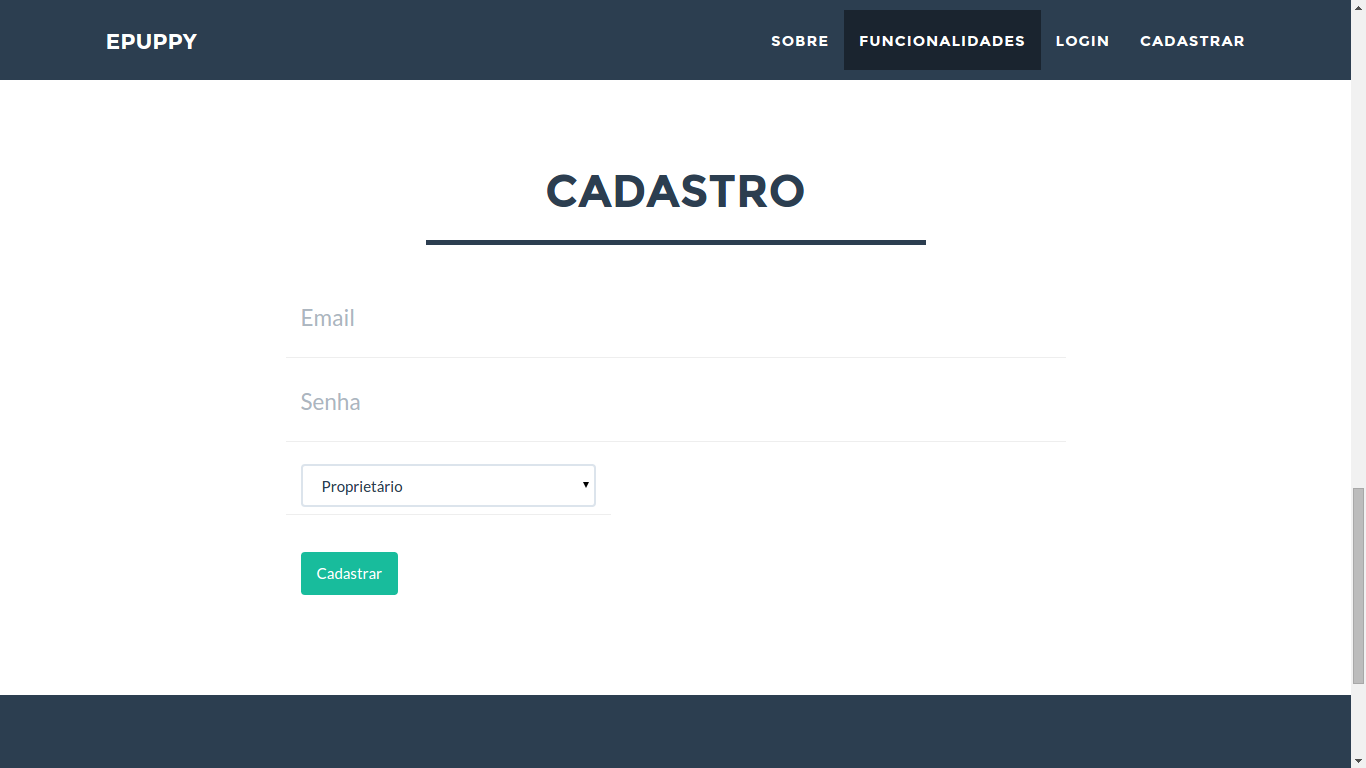
\includegraphics[scale=0.25
	]{imagens/cadastro}
	\caption{Página de cadastro do ePuppy}
	Fonte: Autoria Própria.
	\label{Rotulo}
\end{figure}

\newpage

A principal característica do ePuppy é a integração dos proprietários com clínicas e veterinários, reunindo-os em um único espaço, fazendo disto uma grande rede social interligada, facilitando o cuidado de seu(s) {\it pet}(s). Ao se cadastrar no ePuppy, os proprietários terão direito a adicionar seus animais, seus momentos com ele (seja com fotos ou na descrição de atividades do dia em forma de publicações) e entrar com o pedido de coleiras personalizadas, para que em casos de fuga ou perca, este possa ser facilmente encontrado. Caso o usuário não queira adquirir as coleiras personalizadas, o sistema disponibilizará o {\it QR Code} separadamente, podendo assim ser facilmente impressa conforme o desejo do proprietário.
\begin{figure}[h!]
	\center	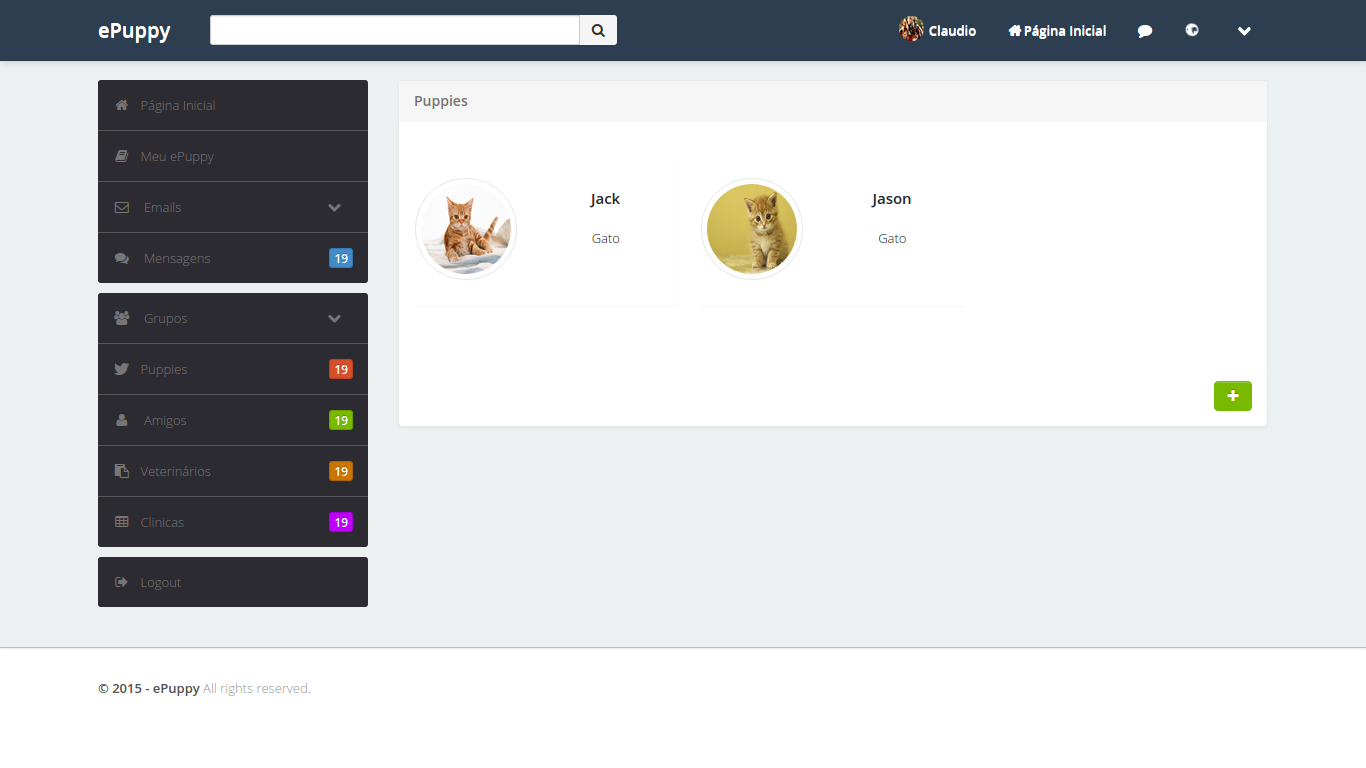
\includegraphics[scale=0.22
	]{imagens/animais1}
	\caption{Página home dos animais de estimação}
	Fonte: Autoria Própria.
	\label{Rotulo}
\end{figure}
\begin{figure}[h!]
	\center	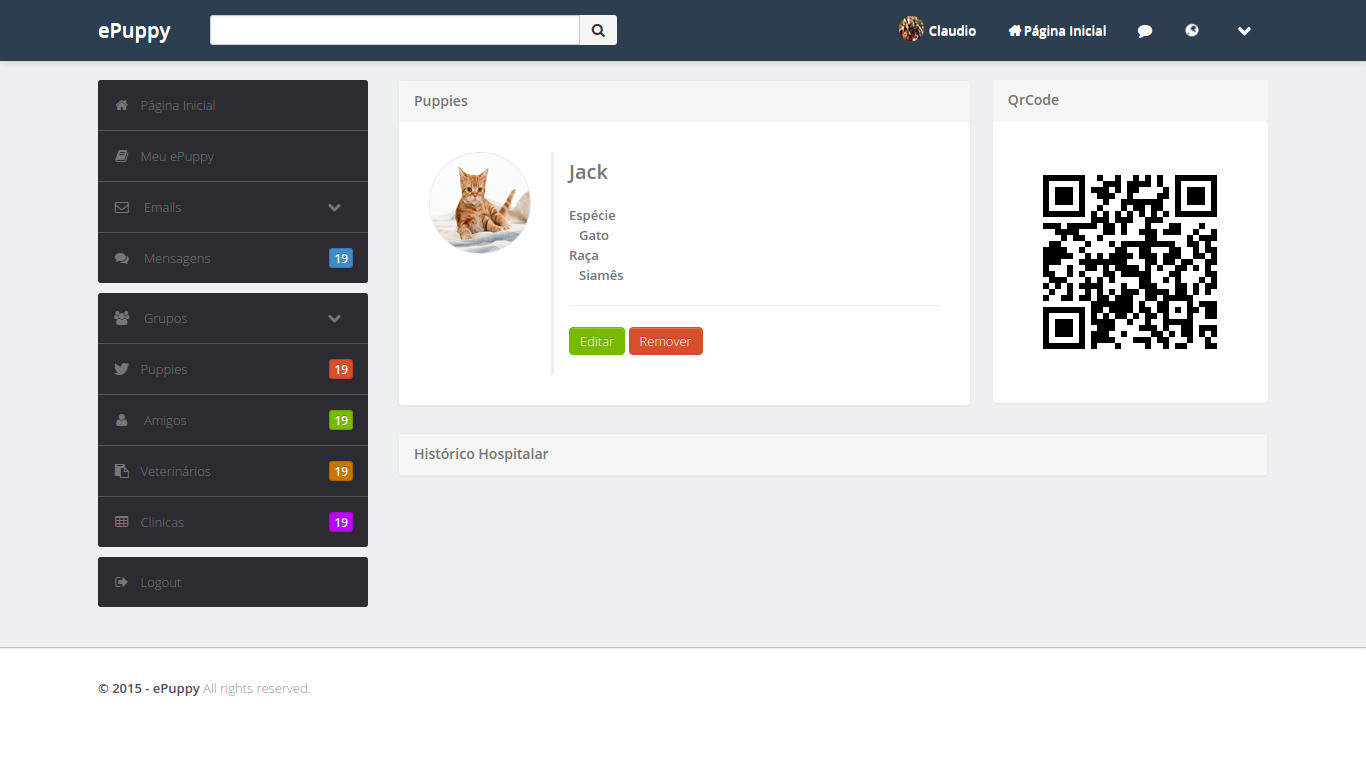
\includegraphics[scale=0.22
	]{imagens/animais2}
	\caption{Página de detalhes dos animais de estimação}
	Fonte: Autoria Própria.
	\label{Rotulo}
\end{figure}

\newpage

É importante destacar que toda a navegação dentro do ePuppy contém o mesmo padrão de navegabilidade e, portanto faz com que as funções sejam notadas claramente pelo usuário e este consiga passar entre todas as {\it urls} do sistema sem precisar de explicação alguma. O usuário poderá ver todos os detalhes de sua conta na sua página principal, na qual, mostrará todos dos seus animais, grupos, amigos e suas principais postagens.

\begin{figure}[h!]
	\center	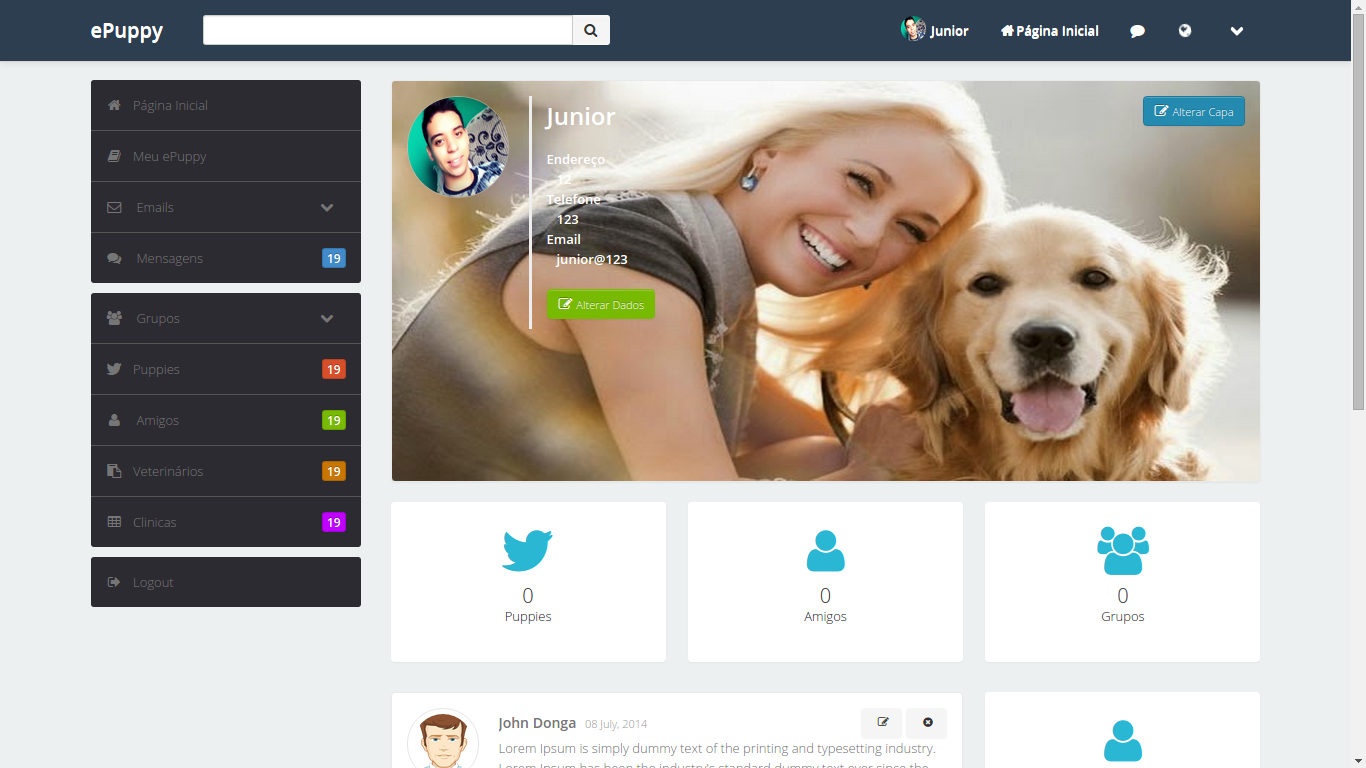
\includegraphics[scale=0.25
	]{imagens/perfil}
	\caption{Perfil do usuário}
	Fonte: Autoria Própria.
	\label{Rotulo}
\end{figure}


A vantagem de utilizar o ePuppy em vez de algum outro programa é a interação que ele propõe dentro do âmbito dos cuidados do animal. Por ser uma grande rede interligada permite que funções de segurança também sirvam para saúde. As coleiras personalizadas, além da função supracitada também servirão para o atendimento dos animais, a medida que o veterinário permitido pelo dono do {\it pet}, pode verificar todo o histórico hospitalar deste, identificando assim, quem fez determinada consulta, a descrição desta e os medicamentos ou cirurgias passadas a estes.


